% !TEX TS-program = XeLaTeX
% !TEX spellcheck = en-US
\documentclass[aspectratio=169]{beamer}

\usetheme{example}

\title{Lecture 6:\\ Unsupervised learning}
\institute{GRA4160: Predictive modelling with machine learning}
\date{February 13th 2025}
\author{Vegard H\o ghaug Larsen}

\begin{document}

\maketitle

% Outline
\begin{frame}
\frametitle{Outline}
\begin{itemize}
    \item Introduction to Dimensionality Reduction
    \item Principal Component Analysis (PCA)
    \item K-Means Clustering
    \item Combining PCA and K-Means
    \item Extensions and Limitations
    %\item Conclusion
\end{itemize}
\end{frame}

% Introduction to Dimensionality Reduction
\begin{frame}
\frametitle{Introduction to Dimensionality Reduction}
\begin{itemize}
    \item What is it?  Reducing the number of variables/features.
    \item Why?  The "Curse of Dimensionality" (overfitting, computation, visualization).
    \item Benefits: Simpler models, faster computation, visualization.
    \item Two main approaches: Feature selection and feature extraction.
    \item Focus: PCA (feature extraction) and K-Means (clustering).
\end{itemize}
\end{frame}

\frame{
      \frametitle{Dimmensionality reduction}
      \begin{center}
            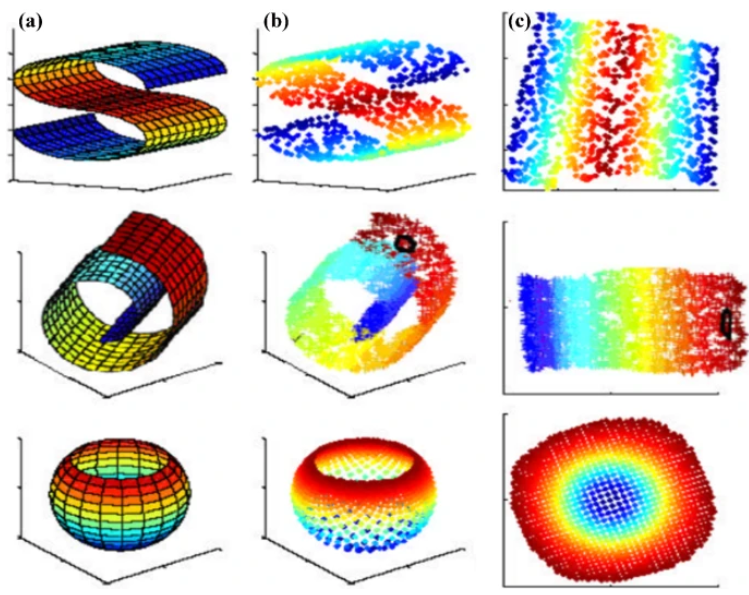
\includegraphics[width=0.5\textwidth]{figures/dim_reduction.png}\\
            \tiny{Source: \href{https://link.springer.com/article/10.1007/s40747-021-00637-x}{Link}}
      \end{center}
}

% PCA: Concept and Goal
\begin{frame}
\frametitle{Principal Component Analysis (PCA): Concept}
\begin{itemize}
    \item Linear dimensionality reduction technique.
    \item Finds new axes (principal components) that maximize variance.
    \item Orthogonal components: Each captures remaining variance.
    \item Unsupervised: Ignores class labels.
    \item Key Idea:  Optimal lower-dimensional representation (maximum variance).
\end{itemize}
\end{frame}

% PCA: Mathematical Foundation
\begin{frame}
\frametitle{PCA: Mathematical Foundation}
\begin{itemize}
    \item Data preparation: Mean-centering, standardization.
    \item Covariance matrix:  Captures feature relationships.
    \item Eigen-decomposition:  $\Sigma \mathbf{v} = \lambda \mathbf{v}$
    \item Eigenvectors: Principal component directions.
    \item Eigenvalues: Variance along each direction.
\end{itemize}
\end{frame}

% PCA: Algorithm Steps
\begin{frame}
\frametitle{PCA: Algorithm Steps}
\begin{enumerate}
    \item Standardize data.
    \item Compute covariance matrix.
    \item Perform eigen-decomposition.
    \item Sort eigenpairs (descending eigenvalues).
    \item Select top $k$ eigenvectors (form projection matrix).
    \item Project data: $\mathbf{Y} = \mathbf{XW}$.
\end{enumerate}
\end{frame}

% PCA: Example and Choosing Components
\begin{frame}
\frametitle{PCA: Example and Choosing Components}
\begin{itemize}
    \item Explained variance: Proportion of variance captured by each component.
    \item Cumulative explained variance:  How much variance is explained by the top *k* components.
    \item Scree plot:  Visualize explained variance vs. component number.
    \item "Elbow" point: Heuristic for choosing *k*.  Trade-off between dimensionality reduction and information loss.
\end{itemize}
\end{frame}

% PCA: Applications
\begin{frame}
\frametitle{PCA: Applications and Use Cases}
\begin{itemize}
    \item Data Visualization (2D/3D projections).
    \item Preprocessing: Feature reduction, noise filtering.
    \item Compression:  Image compression (e.g., Eigenfaces).
    \item Various domains: Genetics, finance, computer vision, etc.
\end{itemize}
\end{frame}

% K-Means: Concept
\begin{frame}
\frametitle{K-Means Clustering: Concept}
\begin{itemize}
    \item Goal: Partition data into $k$ clusters.
    \item Each cluster defined by its centroid (mean).
    \item Each point belongs to the nearest centroid.
    \item "Hard" clustering: Exclusive assignment.
    \item Unsupervised learning.
\end{itemize}
\end{frame}

% K-Means: Objective
\begin{frame}
\frametitle{K-Means: Objective and Properties}
\begin{itemize}
\item Objective: Minimize Within-Cluster Sum of Squares (WCSS).
\item $\min_{S_1,\dots,S_k} \sum_{i=1}^{k} \sum_{\mathbf{x} \in S_i} \|\mathbf{x} - \mu_i\|^2$
\item Centroid: Mean of points in the cluster.
\item Algorithm converges to a local optimum.
\item Assumes convex, roughly spherical clusters.

\end{itemize}
\end{frame}

% K-Means: Algorithm Steps
\begin{frame}
\frametitle{K-Means: Algorithm Steps (Lloyd's Algorithm)}
\begin{enumerate}
    \item Initialization: Choose $k$ initial centroids.
    \item Assignment: Assign points to nearest centroid.
    \item Update: Recalculate centroids.
    \item Iterate: Repeat steps 2 and 3 until convergence.
\end{enumerate}
\end{frame}

% K-Means: Practical Considerations
\begin{frame}
\frametitle{K-Means: Practical Considerations}
\begin{itemize}
    \item Initialization sensitivity: Use k-means++ or multiple runs.
    \item Choosing $k$: Elbow method, silhouette analysis.
    \item Feature scaling: Standardize features.
    \item Outliers: Can distort clusters.
    \item Cluster shape: Assumes spherical clusters.
\end{itemize}
\end{frame}

% K-Means: Use Cases
\begin{frame}
\frametitle{K-Means: Applications and Use Cases}
\begin{itemize}
    \item Market segmentation.
    \item Document clustering.
    \item Image segmentation/compression.
    \item Biology and medicine.
    \item Anomaly detection (points far from centroids).
    \item General exploratory analysis.
\end{itemize}
\end{frame}

% Choosing k
\begin{frame}
\frametitle{Choosing the Number of Clusters (Determining *k*)}
\begin{itemize}
    \item Elbow Method: Plot WCSS vs. *k*, look for "elbow".
    \item Silhouette Analysis: Measure cluster separation.
    \item Domain Knowledge:  Use context.
    \item Validation:  Check for stability and meaning.
\end{itemize}
\end{frame}

% Combining PCA and K-Means
\begin{frame}
\frametitle{Combining PCA and K-Means}
\begin{itemize}
    \item PCA as preprocessing for K-Means.
    \item Benefits:
    \begin{itemize}
        \item Reduces dimensionality and noise.
        \item Speeds up K-Means.
        \item Can improve cluster quality.
        \item Facilitates visualization.
    \end{itemize}
    \item Example: Image clustering.
    \item Caution: Don't reduce dimensions *too* much.
\end{itemize}
\end{frame}

% Extensions and Variants
\begin{frame}
\frametitle{Extensions and Variants of PCA and K-Means}
\begin{itemize}
    \item PCA: Kernel PCA, Sparse PCA, Incremental PCA.
    \item K-Means: K-Means++, K-Medoids, Fuzzy C-Means, Hierarchical Clustering, Gaussian Mixture Models, DBSCAN.
\end{itemize}
\end{frame}

% PCA Limitations
\begin{frame}
\frametitle{Limitations of PCA}
\begin{itemize}
\item  Linearity: PCA is limited in capturing non-linear data.
\item Feature Scaling: Standarization is crucial for unbiased results.
\item Interpretability: Can be difficult with a large number of features
\item Information Loss: Must use explained variance to determine acceptable amount of loss.
\item Outliers: Can signifiantly alter results.
\end{itemize}
\end{frame}

% K-Means Limitations
\begin{frame}
\frametitle{Limitations of K-Means}
\begin{itemize}
\item Choosing $k$: Requires prior knowledge of structure in the data.
\item Cluster shape and size: Assumes spherical clusters of the same size.
\item Sensitivity to initialization: Different starting points can lead to different results.
\item Outliers: Can significantly alter cluster center points.
\end{itemize}
\end{frame}

% Conclusion
\begin{frame}
\frametitle{Conclusion}
\begin{itemize}
    \item \textbf{PCA:} Dimensionality reduction, maximizes variance.
    \item \textbf{K-Means:} Clustering, minimizes within-cluster variance.
    \item \textbf{Use PCA for:} High-dimensional data, visualization, noise reduction.
    \item \textbf{Use K-Means for:}  Finding groups, exploratory analysis.
    \item \textbf{Powerful combination:} PCA + K-Means.
    \item Be aware of limitations and consider extensions.
\end{itemize}
\end{frame}

% \begin{frame}
% \frametitle{References}
% \footnotesize
% \begin{itemize}
%     \item Wikipedia: Principal Component Analysis, K-means Clustering
%     \item Sebastian Raschka (2015): PCA in 3 Steps
%     \item IBM Cloud Learn Hub: What is K-Means Clustering?
%     \item DataCamp Blog (2023): The Curse of Dimensionality in Machine Learning
%     \item Stack Exchange (Cross Validated)
%     \item Brunton et al. (2015): Eigenfaces example

% \end{itemize}

% \end{frame}

\end{document}